\documentclass[12pt]{article}
\usepackage{graphicx}
\usepackage{float}
\usepackage{caption}
\usepackage{subcaption}
\usepackage{fullpage}
\usepackage{lastpage}
\usepackage{fancyhdr}
\usepackage{wrapfig}
\usepackage{lipsum}
\usepackage{mathtools}
\usepackage{amsfonts}
\usepackage{enumitem}
\usepackage{amsmath}
\usepackage{amssymb}
\usepackage{listings}
\usepackage[margin=0.8in]{geometry}

\newcommand{\s}{\hspace{5pt}}
\newcommand{\half}{\frac{1}{2}}
\newcommand{\R}{\mathbb{R}}
\newcommand{\C}{\mathbb{C}}
\newcommand{\p}{\partial}
\newcommand{\mb}{\mathbf}

\newenvironment{m}{\begin{pmatrix}}{\end{pmatrix}}
\newenvironment{e}{\begin{enumerate}[label=(\alph*)]}{\end{enumerate}}

\setlength{\parindent}{0in}

\begin{document}

\title{\vspace{-5ex}Plasma Educational Notes \#1: Ion Acoustic Waves\vspace{-1ex}}
\date{\vspace{-1ex}\today}
\author{Kyle Miller \& Lance Hildebrand}
\maketitle

\section*{Introduction}
Ion acoustic waves (IAWs) are low frequency, longitudinal oscillations of ions in a plasma. They are analogous to sound waves in a neutral gas, but also fundamentally different because of their collisionless nature. In these waves, ions provide the inertia and electrons provide the pressure. The physical picture is as follows: the electrons are pushed out by a pressure gradient. An electric field then develops, so that the ions catch up and then both travel together at the sound speed.

\begin{figure}[H]
	\centering
	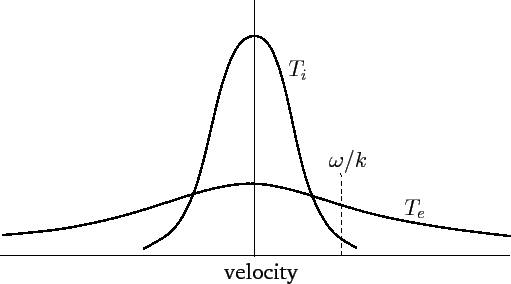
\includegraphics[width=0.5\textwidth]{IAW_dfs}
	\caption{Distribution functions for ions and electrons. The regime of interest is around the dashed line. [1]}
\end{figure}

\section*{Dispersion Relation}
For IAWs, we have inertial electrons and adiabatic ions. First, we look at the Navier-Stokes for the electrons,
\[
	mn_e\frac{\p \mb{v}_e}{\p t}=-en_e\mb{E}-\nabla P_e.
\]
The RHS will be small compared to the other two terms because $m$ and $\omega$ are both small. Neglecting that term and using a ideal equation of state ($P=\gamma n_e T_e$), we can solve for the density to get
\[
	n_e=n_{0e} e^{e\phi/T_e},
\]
where we use $\gamma=1$ because electrons are inertial. Linearizing we get
\[
	\tilde{n}_e=n_{0e}\frac{e\tilde{\phi}}{T_e}.
\]
Now we look at the ion equations. We write Navier-Stokes as
\[
\frac{\p \tilde{\mb{v}}_i}{\p t}=-\frac{q}{m_i}\nabla \tilde{\phi},
\]
and the continuity equation as
\[
	\frac{\p \tilde{n}_i}{\p t}+\nabla \cdot [n_{0i}\tilde{\mb{v}}_i]=0.
\]
Taking the divergence of the former and the time derivative of the latter, combining and plugging into Poisson's Equation, we get
\[
	\tilde{n}_i=\frac{n_{0e} e \tilde{\phi}}{Z T_e}-\frac{\nabla ^2 \tilde{\phi}}{4 \pi e Z}.
\]
We now plug this back into the time derivative of the continuity equation and simplify to get the IAW equation:
\[
	\frac{\p ^2}{\p t^2} \left[ \tilde{\phi} - \frac{1}{k_D^2}\nabla ^2 \tilde{\phi}\right]-\frac{Z T_e}{m_i}\nabla ^2 \tilde{\phi} =0.
\]
Now we assume plane wave solutions and solve to get the dispersion relation
\[
	\omega=\frac{k c_s}{\sqrt{1+(k/k_D)^2}},
\]
where $c_s=\sqrt{\frac{Z T_e}{m_i}}$ is the sound speed.

\begin{figure}[H]
	\centering
	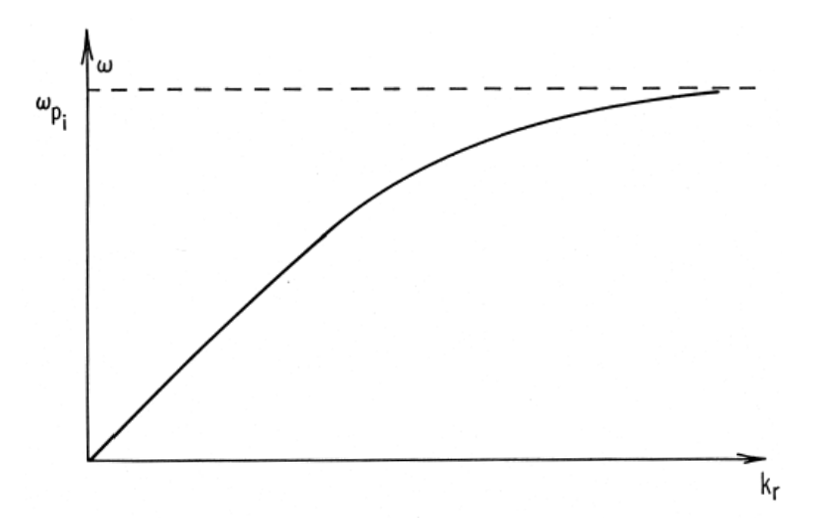
\includegraphics[width=0.5\textwidth]{IAW_DR}
	\caption{Dispersion relation for IAWs}
\end{figure}

\section*{Parameters}
\begin{e}
	\item Vary the temperature ratio. Well defined IAW occur in the low frequency regime. We can write, to first order, $\frac{\omega}{k}=\sqrt{\frac{Z T_e}{T_i}}\bar{v}_i$. So we need $\frac{T_e}{T_i}\gtrsim 10$ for well-defined IAWs.
	
	\item Vary the mass ratio. This will change the ratio of the thermal velocities of the electrons and ions. As the mass of the ions is increased, the smaller $\bar{v}_i$ will be and thus the smaller $\frac{\omega}{k}$ can be. So IAWs will generally be better defined for heavy ions.
\end{e}

\section*{References}
[1] Fitzpatrick, R. (2016) \textit{Ion Acoustic Waves}, Retrieved from\\ https://farside.ph.utexas.edu/teaching/plasma/Plasma/node112.html


\end{document}
